\documentclass[a4paper, 11pt]{article}

% DEFINIËREN CODERING
\usepackage[utf8]{inputenc}

% DEFINIËREN BLAD
\usepackage[
top=20mm,
bottom=20mm,
left=20mm,
right=20mm,
heightrounded,
]{geometry}
\usepackage{lastpage}
\usepackage{fancyhdr}
%\pagestyle{fancy}
\fancyhead[L]{}
\fancyhead[C]{}
\fancyhead[R]{}
\fancyfoot[L]{}
\fancyfoot[C]{\thepage}
\fancyfoot[R]{}
\renewcommand{\headrulewidth}{0pt}
\renewcommand{\footrulewidth}{.4pt}
\setlength{\headheight}{13.6pt}
\setlength{\parindent}{1cm}

% MEDIA
% Tabellen
\usepackage{array}
\newcolumntype{L}[1]{>{\raggedright\let\newline\\\arraybackslash\hspace{0pt}}m{#1}}
\newcolumntype{C}[1]{>{\centering\let\newline\\\arraybackslash\hspace{0pt}}m{#1}}
\newcolumntype{R}[1]{<{\raggedleft\let\newline\\\arraybackslash\hspace{0pt}}m{#1}}
\usepackage{stackengine}
\newcommand\xrowht[2][0]{\addstackgap[.5\dimexpr#2\relax]{\vphantom{#1}}}
\usepackage{tabularx}
\usepackage{multirow}
\usepackage{hhline}
\usepackage{float}
\usepackage[table]{xcolor}
% Afbeeldingen
\usepackage{graphicx}
% Figuren
\usepackage{tikz}
% URLS
\usepackage{hyperref}
% Comments
\usepackage{comment}

% WISKUNDE
% Basis
\usepackage{amsmath}
\usepackage{amssymb}
\usepackage{amsthm}
\usepackage{mathtools}
% Aanpassing
\usepackage{dsfont}   % Voor de natuurlijke, gehele, rationele, reële, complexe getallen => ``$\mathfb{}$''
\usepackage{mathdots} % Voor betere puntjes
\usepackage{esvect}   % Voor betere vectorpijltjes => ``$\vv{}$''
\usepackage{textcomp} % Nodig om gensymb correct te laten werken
\usepackage{gensymb}  % Invoegen van enkele symbolen => ``\degree ; \celcius ; \perthousand ; \ohm ; \micro''
\usepackage{cancel}   % Voor het beter doorstrepen van zaken => ``\cancel ; \bcancel ; \xcancel''
\usepackage{esint}    % Meervoudige kringintegralen

\newcommand{\naar}{\,$\rightarrow$\,}
\newcommand{\ppp}{\ldots}
\renewcommand{\empty}{$\varnothing$}
\newcommand{\of}{$\cup$\;}
\newcommand{\<}{\scriptsize\textless\normalsize}
\renewcommand{\>}{\scriptsize\textgreater\normalsize}

% Voorblad
\title{Programmeerproject 2:\\ Specificatie voor Ontwikkelaars - Besturingssysteem Modeltreinen		
	\author{Jonas Br\"ull, 0587194\\ Jonas.Simon.E.Brull@vub.be\\}
	\date{Academiejaar 2024-2025\\Vrije Universiteit Brussel}
	\thanks{\texttt{\url{https://github.com/Jonas-Bruell/besturingssysteem-modeltreinen}}}
}

% =================================================================================================
\begin{document}

\pagenumbering{gobble}
\maketitle
\newpage

\pagenumbering{gobble}
\tableofcontents
\newpage

\pagestyle{fancy}
\setcounter{page}{1}
\pagenumbering{arabic}

% =================================================================================================
\section{Introductie} % ===========================================================================
Dit document beschrijft het ontwerp van de implementatie van een Modeltrein Software Toepassing in de programmeertaal Racket. Het is een deel van het opleidingsonderdeel ``Programmeerproject 2''.\\
\newline
Het onderwerp van het project is de ontwikkeling van een controlesysteem voor een modelspoor. De modeltreinen kunnen volledig digitaal aangestuurd worden door een extern programma aangestuurd met digitale commando’s. Digitale locomotieven gebruiken het elektrisch circuit op de sporen als een datacommunicatiebus. Niet alleen de snelheid van de locomotieven wordt op deze manier digitaal
geregeld, maar ook andere functionaliteiten zoals het veranderen van wissels\\
\newline
Tijdens deze opdracht wordt een controlesysteem ontwikkeld om modeltreinen aan te sturen. Het is de
bedoeling dat tegen het einde van het academiejaar een systeem ontwikkeld werd dat gebruikers
toelaat vanaf hun computer treinen over een modelspoor te laten rijden.\\
\newline
Het project bestaat uit drie grote componenten:
\begin{itemize}
	\item Een Command Station (Z21) dat de verschillende elementen van het modelspoor aanstuurt. Dit Command Station communiceert met de hardware via het Digital Command Control (DCC) protocol. De software hiervoor zit reeds ingebouwd in het Command Station. Het Command Station is aan te sturen door er via het netwerk commando’s naar te sturen door middel van de Z21-bibliotheek.
	\item Infrabel is de component die instaat voor de communicatie tussen de software en de
	modelbouwhardware (detectie van treinen en aansturing van treinen en wissels) en het
	doorlopend beheer van de infrastructuur (bv. automatisch remsysteem). Dit is deel van de infrastructuur en moet permanent draaien. Infrabel kan draaien op een computer of op een Raspberry Pi (een kleine gelimiteerde computer).
	\item NMBS en de grafische interface (GUI). NMBS staat in voor de functionaliteit die geen
	logisch onderdeel is van de infrastructuur maar er bovenop bouwt, zoals een grafische
	interface, het uitstippelen van trajecten of het opstellen van tijdstabellen. NMBS draait
	op je eigen computer en communiceert met Infrabel. Naar het einde van het project toe
	zal die communicatie via een netwerkverbinding (TCP) dienen te gebeuren.
\end{itemize}
Zowel de Infrabel module, als de Provider module zullen steunen op een railway module, deze de fysieke spoorwegopstelling (of diens simulator) modeleert en deze steeds dezelfde staat zal hebben.

% =================================================================================================
\newpage
\section{Globaal afhankelijkheidsdiagram} % =======================================================
Het besturingssysteem bestaat uit twee grote componenten: "infrabel" en "provider".\\De "infrabel" component wordt via INFRABEL tot een object gemaakt en is de centrale server deze de modelspoorlijn aanstuurt. De "provider" component is een template die via "NMBS", "DB", ... verschillende objecten wordt gemaakt, en deze de clients vormen, deze via een TCP verbinding met INFRABEL communiceren.\\
Zowel "infrabel" als "provider" hebben een gemeenschappelijke abstractielaag, "railway", deze zorgt voor consistentie tussen beide componenten, zonder aan elkaar verbonden te zijn. Beide componenten hebben hun eigen, afzonderlijke "railway".
\begin{figure}[h]
	\begin{center}
		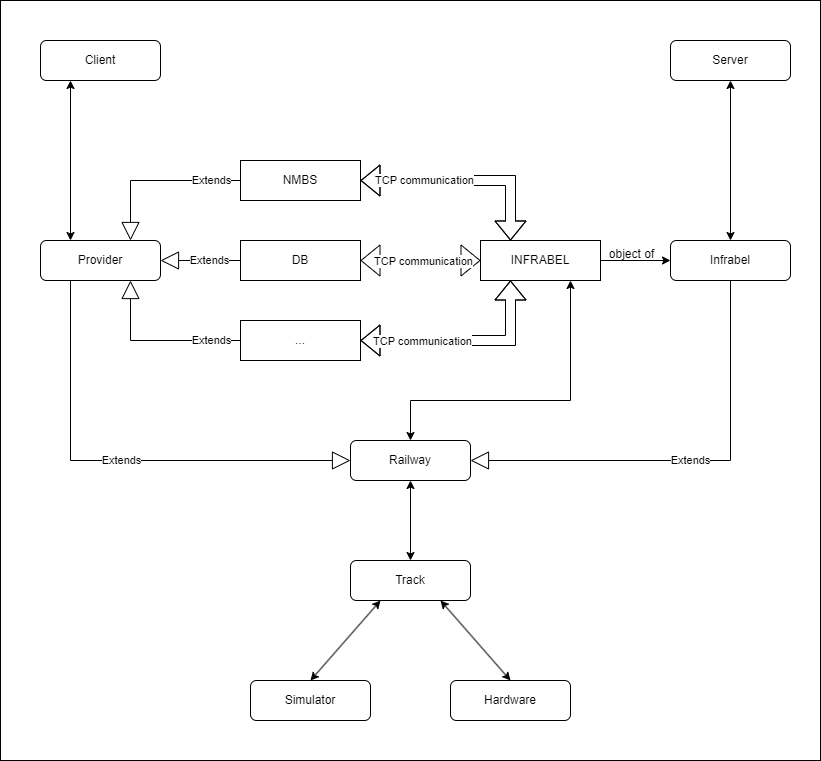
\includegraphics[scale=.5]{Afhankelijkheidsdiagrammen/global.png}
		\caption{Globaal, versimpeld afhankelijkheidsdiagram}
	\end{center}
\end{figure}

% =================================================================================================
\newpage
\section{Track} % =================================================================================
De track-module is de abstractielaag over de interfaces van de simulator en de hardware. Deze module bevat de abstracties voor de verschillende hardware-componenten die de modelspoorweg bezit. Deze abstractielaag maakt dit project onafhankelijk van de externe libraries.

\subsection{afhankelijkheidsdiagram} % ++++++++++++++++++++++++++++++++++++++++++++++++++++++++++++
\begin{figure}[h]
	\begin{center}
		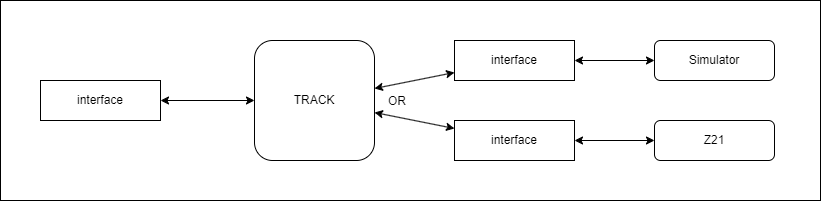
\includegraphics[scale=.5]{Afhankelijkheidsdiagrammen/track.png}
		\caption{Afhankelijkheidsdiagram van de track-module}
	\end{center}
\end{figure}

% Implemented, Tested, Documented ~~~~~~~~~~~~~~~~~~~~~~~~~~~~~~~~~~~~~~~~~~~~~~~~~~~~~~~~~~~~~~~~~
\subsection{interface.rkt} % ++++++++++++++++++++++++++++++++++++++++++++++++++++++++++++++++++++++
De \texttt{Track} klasse is een interface die kan worden opgeroepen vanuit andere modules van het besturingssysteem. Deze klasse bevat alle nodige operaties om de hardware-componenten van de spoorweg aan te sturen.
\begin{table}[H]
	\begin{center}
		{\rowcolors{2}{gray!50!white!50}{white!100}
		\begin{tabular}{|l l|}
			\hline
			\textbf{Naam + signatuur} & \textbf{Uitleg}\\
			\hline
			\texttt{make-object} : (\textit{symbol} \of \empty, \textit{symbol} \of \empty \naar \textit{Track}) & Constructor\\
			\hline
			% setup
			\texttt{get-architecture} : (\empty \naar \textit{symbol}) & Geeft de architectuur van de track weer.\\
			\texttt{get-version} : (\empty \naar \textit{symbol}) & Geeft de versie van de track weer.\\
			\texttt{get-versions} : (\empty \naar \textit{pair}) & Geeft verschillende versies van track weer.\\
			\texttt{config!} : (\textit{symbol}, \textit{symbol} \naar \empty) & Configureert track met architecture \& versie.\\
			\texttt{start} : (\empty \naar \empty) & Start de Track module.\\
			\texttt{stop} : (\empty \naar \empty) & Start de Track module.\\
			% loco
			\texttt{add-loco} : (\textit{symbol}, \textit{symbol}, \textit{symbol} \naar \empty) & Plaatst een locomotief op de Track.\\
			\texttt{get-loco-speed} : (\textit{symbol} \naar \textit{number}) & Geeft de snelheid van de gegeven locomotief.\\
			\texttt{set-loco-speed!} : (\textit{symbol}, \textit{number} \naar \empty) & Zet de snelheid naar de opgegeven snelheid.\\
			% detecion-blocks
			\texttt{get-detection-block-ids} : (\empty \naar \textit{pair}) & Geeft lijst van detection-block ids terug.\\
			\texttt{get-occupied-detection-blocks} : (\empty \naar \textit{pair}) & Geeft lijst van bezette detection-blocks.\\
			% switches
			\texttt{get-switch-ids} : (\empty \naar \textit{pair}) & Geeft lijst van wissels terug.\\
			\texttt{get-switch-position} : (\textit{symbol} \naar \textit{number}) & Geeft positie van gegeven wissel.\\
			\texttt{set-switch-position!} : (\textit{symbol}, \textit{number} \naar \empty) & Zet positie van opgegeven wissel.\\
			% crossings
			\texttt{set-crossing-position!} : (\textit{symbol}, \textit{symbol} \naar \empty) & Zet de positie van de opgegeven overweg.\\
			% lights
			\texttt{set-sign-code!} : (\textit{symbol}, \textit{symbol} \naar \empty) & Zet het signaal van het opgegeven licht.\\
			\hline
		\end{tabular}}
		\caption{Operaties van de Track klasse}
	\end{center}
\end{table}

% =================================================================================================
\newpage
\section{Railway} % ===============================================================================
De railway-module houdt ten allen tijden de staat van de fysieke modelspoorweg bij. Deze module bestaat uit verschillende atomaire abstracties van de verschillende hardware-componenten, die de modelspoorweg bezit, deze allemaal aangestuurd worden vanuit de railway-klasse.
\newline\\
De railway-module is niet afhankelijk van de track-module, maar abstraheert deze door zijn oproepen te doen naar een "connection". Deze connection kan de track-interface zijn, maar bijvoorbeeld ook een client voor een provider, op op deze manier messages naar infrabel te sturen.
\newline\\
De railway-module bevat ook een "controle-panel", een heel basic gui, waarmee de wissels, lichten, overwegen, treinen en detectieblokken kunnen worden aangestuurd of uitgelezen. Deze gui is enkel bedoeld voor testdoeleinden en zal niet worden gebruikt in de uiteindelijke software.

% =================================================================================================
\subsection{afhankelijkheidsdiagram} % ============================================================
\begin{figure}[h]
	\begin{center}
		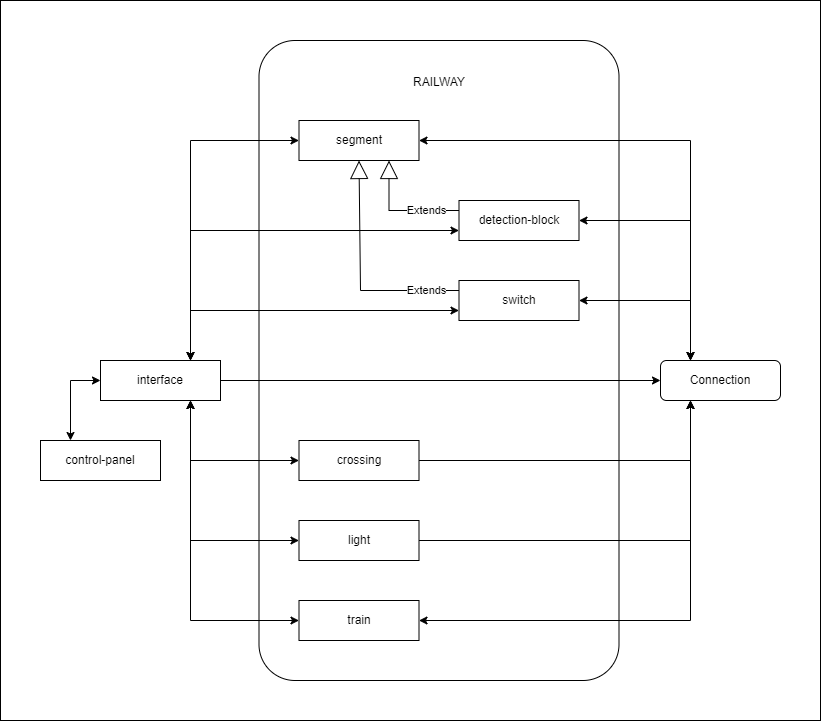
\includegraphics[scale=.5]{Afhankelijkheidsdiagrammen/railway.png}
		\caption{Afhankelijkheidsdiagram van de railway-module}
	\end{center}
\end{figure}

\subsection{interface.rkt} % ++++++++++++++++++++++++++++++++++++++++++++++++++++++++++++++++++++++
De \texttt{Railway} klasse is het startpunt van railway-module van de software en functioneert tevens ook als een interface. Om een digitaal equivalent van de staat van de modelspoorweg bij te houden, bezit deze interface hiervoor ook de nodige getters en setters.

\newpage

\begin{table}[H]
	\begin{center}
		{\rowcolors{2}{gray!50!white!50}{white!100}
		\begin{tabular}{|l l|}
			\hline
			\textbf{Naam + signatuur} & \textbf{Uitleg}\\
			\hline
			\texttt{make-object} : (\textit{Connection} \naar \textit{Railway}) & Constructor\\
			\hline
			% control-panel
			\texttt{start-control-panel} : (\empty \naar \empty) & Start het controlepaneel van de railway.\\
			% segments
			\texttt{get-segment-ids} : (\empty \naar \textit{pair}) & Geeft lijst van segmenten.\\
			\texttt{get-segment-next} : (\textit{symbol} \naar \textit{symbol}) & Geeft volgende (wijzerzin) segment terug.\\
			\texttt{get-segment-prev} : (\textit{symbol} \naar \textit{symbol}) & Geeft vorige (wijzerzin) segement terug. \\
			\texttt{get-segment-state} : (\textit{symbol} \naar \textit{symbol}) & Geeft status weer van gegeven segment.\\
			\texttt{set-segment-state!} : (\textit{symbol}, \textit{symbol} \naar \empty) & Zet status van het opgegeven segment.\\
			% detection-blocks
			\texttt{get-detection-block-ids} : (\empty \naar \textit{pair}) & Geeft lijst van detectieblokken.\\
			\texttt{get-detection-block-next} : (\textit{symbol} \naar \textit{symbol}) & Geeft volgende (wijzerzin) detectieblok.\\
			\texttt{get-detection-block-prev} : (\textit{symbol} \naar \textit{symbol}) & Geeft vorige (wijzerzin) detectieblok.\\
			\texttt{get-detection-block-state} : (\textit{symbol} \naar \textit{symbol}) & Geeft status weer van gegeven detectieblok.\\
			\texttt{set-detection-block-state!} : (\textit{symbol} \naar \empty) & Zet status van gegeven detectieblok.\\
			% switches
			\texttt{get-switch-ids} : (\empty \naar \textit{pair}) & Geeft lijst van wissels terug.\\
			\texttt{get-switch-next} : (\textit{symbol} \naar \textit{pair}) & Geeft lijst volgende (2-segmenten kant) segmenten.\\
			\texttt{get-switch-next-left} : (\textit{symbol} \naar \textit{symbol}) & Geeft linker volgende (2-segmenten kant) segment.\\
			\texttt{get-switch-next-right} : (\textit{symbol} \naar \textit{symbol}) & Geeft rechter volgende (2-segmenten kant) segment.\\
			\texttt{get-switch-prev} : (\textit{symbol} \naar \textit{symbol}) & Geeft vorige (1-segment kant) segment.\\
			\texttt{get-switch-state} : \textit{symbol} \naar \textit{symbol}) & Geeft status weer van gegeven wissel.\\
			\texttt{set-switch-state!} : (\textit{symbol}, \textit{symbol} \naar \empty) & Zet status van het opgegeven wissel.\\
			\texttt{get-switch-position} : (\textit{symbol} \naar \textit{symbol}) & Geeft postitie weer van gegeven wissel.\\
			\texttt{set-switch-position!} : (\textit{symbol} \textit{symbol} \naar \empty) & Update gegeven wissel met gegeven positie.\\
			% crossings
			\texttt{get-crossing-ids} : (\empty \naar \textit{pair}) & Geeft lijst van overwegen.\\
			\texttt{get-crossing-segments}: (\textit{symbol} \naar \textit{pair}) & Geeft lijst met segmenten tussen de overweg.\\
			\texttt{get-crossing-position} : (\textit{symbol} \naar \textit{symbol}) & Geeft positie weer van slagbomen gegeven overweg.\\
			\texttt{set-crossing-position!} : (\textit{symbol} \textit{symbol} \naar \empty) & Update gegeven overweg naar gegeven positie\\
			% lights
			\texttt{get-light-ids} : (\empty \naar \textit{pair}) & Geeft lijst van lichten\\
			\texttt{get-light-segment} : (\textit{symbol} \naar \textit{symbol}) & Geeft segment terug waaraan licht grenst.\\
			\texttt{get-light-signal} : (\textit{symbol} \naar \textit{symbol}) & Geeft signaal weer van gegeven licht\\
			\texttt{set-light-signal!} : (\textit{symbol} \textit{symbol} \naar \empty) & Update gegeven licht met gegeven signaal\\
			% trains
			\texttt{get-train-ids} : (\empty \naar \textit{pair}) & Geeft lijst van treinen\\
			\texttt{get-train-speed} : (\textit{symbol} \naar \textit{symbol}) & Geeft snelheid weer van gegeven trein\\
			\texttt{set-train-speed!} : (\textit{symbol} \textit{symbol} \naar \empty) & Update gegeven trein met gegeven snelheid\\
			\hline
		\end{tabular}}
		\caption{Operaties van de Railway klasse}
	\end{center}
\end{table}

% Implemented, Tested, Documented ~~~~~~~~~~~~~~~~~~~~~~~~~~~~~~~~~~~~~~~~~~~~~~~~~~~~~~~~~~~~~~~~~
\subsection{crossing.rkt} % +++++++++++++++++++++++++++++++++++++++++++++++++++++++++++++++++++++++
De \texttt{Crossing} klasse is de atomaire abstractie van een spoorwegoverweg. De constructor neemt als argumenten het \texttt{id} van de overweg, een \lq\texttt{connection}' (communicatie naar ondergelegen laag) en een lijst van spoorwegsegmenten waarover deze overweg brugt. Het openen en sluiten van deze overweg neemt wat tijd in beslag, waartussen de overweg als status \lq\texttt{pending}' heeft.
\begin{table}[H]
	\begin{center}
		{\rowcolors{2}{gray!50!white!50}{white!100}
		\begin{tabular}{|l l|}
			\hline
			\textbf{Naam + signatuur} & \textbf{Uitleg}\\
			\hline
			\texttt{make-object} : (\textit{symbol Object list} \naar \textit{Crossing}) & Constructor\\
			\hline
			\texttt{get-id} : (\empty \naar \textit{symbol}) & Geeft het \texttt{id} van de overweg.\\
			\texttt{get-state} : (\empty \naar \textit{symbol}) & Geeft de \texttt{status} van de overweg.\\
			\texttt{get-segments} : (\empty \naar \textit{list}) & Geeft de segmenten waarover de overweg brugt.\\
			\texttt{set-state!} : (\textit{symbol} \naar \empty) & Open of sluit de overweg adhv een status.\\
			\hline
		\end{tabular}}
		\caption{Operaties van de Railway/Crossing klasse}
	\end{center}
\end{table}

% Implemented, Tested, Documented ~~~~~~~~~~~~~~~~~~~~~~~~~~~~~~~~~~~~~~~~~~~~~~~~~~~~~~~~~~~~~~~~~
\subsection{detection-block.rkt} % ++++++++++++++++++++++++++++++++++++++++++++++++++++++++++++++++
De \texttt{Detection-block} klasse is de atomaire abstractie van een detectieblok. Deze is een uitbreiding van de \texttt{Segment} klasse. De constructor neemt als argumenten het \texttt{id} van het detectieblok, een \lq\texttt{connection}' (communicatie naar ondergelegen laag) en de twee andere spoorwegelementen waartussen dit detectieblok zich bevindt. De status van het detectieblok kan ofwel \texttt{free}, ofwel \texttt{reserved}, ofwel \texttt{occupied} zijn.
\begin{table}[H]
	\begin{center}
		{\rowcolors{2}{gray!50!white!50}{white!100}
		\begin{tabular}{|l l|}
			\hline
			\textbf{Naam + signatuur} & \textbf{Uitleg}\\
			\hline
			$\begin{matrix}
				\texttt{make-object} & (\textit{symbol Object symbol symbol} \\
				& \rightarrow \textit{Detection-block})\\
			\end{matrix}$
			& Constructor \\
			\hline
			\texttt{get-id} : (\empty \naar \textit{symbol}) & Geeft het \texttt{id} van het detectieblok.\\
			\texttt{get-state} : (\empty \naar \textit{symbol}) & Geeft de \texttt{status} van het detectieblok.\\
			\texttt{get-next} : (\empty \naar \textit{symbol}) & Geeft het volgende spoorwegelement weer.\\
			\texttt{get-prev} : (\empty \naar \textit{symbol}) & Geeft het vorige spoorwegelement weer.\\
			\texttt{set-state!} : (\textit{symbol} \naar \textit{boolean}) & 
			$\begin{matrix*}[l]
				\text{Update de \texttt{status} van het detectieblok.}\\
				\text{• False wanneer \texttt{(set-state! 'reserved)}}\\
				\text{\quad indien \texttt{Detection-block} gereserveerd.}\\
			 	\text{• False wanneer \texttt{(set-state! 'reserved)}}\\
			  \text{\quad indien \texttt{Detection-block} occupied.}\\
			 	\text{• False wanneer \texttt{(set-state! 'occupied)}}\\
			  \text{\quad indien \texttt{Detection-block} occupied.}\\
		\end{matrix*}$\\
		\hline
		\end{tabular}}
		\caption{Operaties van de Railway/Detection-block klasse}
	\end{center}
\end{table}

% Implemented, Tested, Documented ~~~~~~~~~~~~~~~~~~~~~~~~~~~~~~~~~~~~~~~~~~~~~~~~~~~~~~~~~~~~~~~~~
\subsection{light.rkt} % ++++++++++++++++++++++++++++++++++++++++++++++++++++++++++++++++++++++++++
De \texttt{Light} klasse is de atomaire abstractie van een licht. De constructor neemt als argumenten het \texttt{id} van het licht, een \lq\texttt{connection}' (communicatie naar ondergelegen laag) en een spoorwegsegment waarover dit licht gaat. Het licht kan de volgende statussen hebben: \texttt{Hp0}, \texttt{Hp1}, \texttt{Hp0+Sh0}, \texttt{Ks1+Zs3}, \texttt{Ks2}, \texttt{Ks2+Zs3}, \texttt{Sh1}, \texttt{Ks1+Zs3+Zs3v}.
\begin{table}[H]
	\begin{center}
		{\rowcolors{2}{gray!50!white!50}{white!100}
		\begin{tabular}{|l l|}
			\hline
			\textbf{Naam + signatuur} & \textbf{Uitleg}\\
			\hline
			\texttt{make-object} : (\textit{symbol Object symbol} \naar \textit{Light}) & Constructor\\
			\hline
			\texttt{get-id} : (\empty \naar \textit{symbol}) & Geeft het \texttt{id} van het licht.\\
			\texttt{get-signal} : (\empty \naar \textit{symbol}) & Geeft het \texttt{signal} van het licht.\\
			\texttt{get-segment} : (\empty \naar \textit{symbol}) & Geeft het segment waarover het licht gaat.\\
			\texttt{set-signal!} : (\textit{symbol} \naar \empty) & Update het signaal van het licht.\\
			\hline
		\end{tabular}}
		\caption{Operaties van de Railway/Light klasse}
	\end{center}
\end{table}

% Implemented, Tested, Documented ~~~~~~~~~~~~~~~~~~~~~~~~~~~~~~~~~~~~~~~~~~~~~~~~~~~~~~~~~~~~~~~~~
\subsection{segment.rkt} % ++++++++++++++++++++++++++++++++++++++++++++++++++++++++++++++++++++++++
De \texttt{Segment} klasse is de atomaire abstractie van een spoorwegsegment. De constructor neemt als argumenten het \texttt{id} van het spoorwegsegment, een \lq\texttt{connection}' (communicatie naar ondergelegen laag) en de twee andere spoorwegelementen waartussen dit spoorwegsegment zich bevindt. De status van het spoorwegsegment kan ofwel \texttt{free}, ofwel \texttt{reserved} zijn.
\begin{table}[H]
	\begin{center}
		{\rowcolors{2}{gray!50!white!50}{white!100}
		\begin{tabular}{|l l|}
			\hline
			\textbf{Naam + signatuur} & \textbf{Uitleg}\\
			\hline
			\texttt{make-object} : (\textit{symbol Object symbol symbol} \naar \textit{Segment}) & Constructor\\
			\hline
			\texttt{get-id} : (\empty \naar \textit{symbol}) & Geeft het \texttt{id} van het segment.\\
			\texttt{get-state} : (\empty \naar \textit{symbol}) & Geeft de \texttt{status} van het segment.\\
			\texttt{get-next} : (\empty \naar \textit{symbol}) & Geeft het volgende spoorwegelement weer.\\
			\texttt{get-prev} : (\empty \naar \textit{symbol}) & Geeft het vorige spoorwegelement weer.\\
			\texttt{set-state!} : (\textit{symbol} \naar \textit{boolean}) &
			$\begin{matrix*}[l]
				\text{Update de \texttt{status} van het segment.}\\
				\text{False wanneer \texttt{(set-state! 'reserved)}}\\
				\text{indien \texttt{Segment} reeds gereserveerd.}\\
			\end{matrix*}$\\
			\hline
		\end{tabular}}
		\caption{Operaties van de Railway/Segment klasse}
	\end{center}
\end{table}

% Implemented, Tested, Documented ~~~~~~~~~~~~~~~~~~~~~~~~~~~~~~~~~~~~~~~~~~~~~~~~~~~~~~~~~~~~~~~~~
\subsection{switch.rkt} % +++++++++++++++++++++++++++++++++++++++++++++++++++++++++++++++++++++++++
De \texttt{Switch} klasse is de atomaire abstractie van een spoorwegwissel. Deze is een uitbreiding van de \texttt{Segment} klasse. De constructor neemt als argumenten het \texttt{id} van de wissel, een \lq\texttt{connection}' (communicatie naar ondergelegen laag) en de andere spoorwegelementen waartussen deze wissel zich bevindt, de ingaande als \texttt{symbol} en de uitgaande als een \texttt{cons}-cel van \texttt{symbol}s. De positie van de wissel kan ofwel \texttt{left}, ofwel \texttt{right}, zijn.
\begin{table}[H]
	\begin{center}
		{\rowcolors{2}{gray!50!white!50}{white!100}
		\begin{tabular}{|l l|}
			\hline
			\textbf{Naam+ signatuur} & \textbf{Uitleg}\\
			\hline
			\texttt{make-object} : (\textit{symbol Object symbol pair} \naar \textit{Switch}) & Constructor\\
			\hline
			\texttt{get-id} : (\empty \naar \textit{symbol}) & Geeft het \texttt{id} van de wissel.\\
			\texttt{get-state} : (\empty \naar \textit{symbol}) & Geeft de \texttt{status} van de wissel.\\
			\texttt{get-position} : (\empty \naar \textit{symbol}) & Geeft de \texttt{position} van de wissel\\
			\texttt{get-next-left} : (\empty \naar \textit{symbol}) & Geeft het volgende spoorwegelement weer.\\
			\texttt{get-next-right} : (\empty \naar \textit{symbol}) & Geeft het volgende spoorwegelement weer.\\
			\texttt{get-prev} : (\empty \naar \textit{symbol}) & Geeft het vorige spoorwegelement weer.\\
			\texttt{set-state!} : (\textit{symbol} \naar \empty) & Update de \texttt{status} van de wissel.\\
			\texttt{set-position!} : (\textit{symbol} \naar \empty) & Update de status van de wissel\\
			\hline
		\end{tabular}}
		\caption{Operaties van de Railway/Switch klasse}
	\end{center}
\end{table}

\begin{comment}

\subsection{switch-3way.rkt} % ++++++++++++++++++++++++++++++++++++++++++++++++++++++++++++++++++++
De \texttt{Switch-3way} klasse is de atomaire abstractie van een spoorwegwissel deze van 3 sporen laat samenkomen tot 1 spoor. Deze klasse is een uitbreiding is van de \texttt{Switch} klasse. De constructor neemt als argumenten het \texttt{id} van de wissel, een \lq\texttt{connection}' (communicatie naar ondergelegen laag) en de andere spoorwegelementen waartussen deze wissel zich bevindt, de ingaande als \texttt{symbol} en de uitgaande als een \texttt{list} van \texttt{symbol}s. De positie van de wissel kan ofwel \texttt{left}, ofwel \texttt{middle}, ofwel \texttt{right}, zijn.
\begin{table}[H]
	\begin{center}
		{\rowcolors{2}{gray!50!white!50}{white!100}
		\begin{tabular}{|l l l|}
			\hline
			\textbf{Naam} & \textbf{Signatuur} & \textbf{Uitleg}\\
			\hline
			\texttt{make-object} & (\textit{symbol Object symbol list} \naar \textit{Switch}) & Constructor\\
			\hline
			\texttt{get-id} & (\empty \naar \textit{symbol}) & Geeft het \texttt{id} van de 3-wegs wissel.\\
			\texttt{get-state} & (\empty \naar \textit{symbol}) & Geeft de \texttt{status} van de 3-wegs wissel.\\
			\texttt{get-position} & (\empty \naar \textit{symbol}) & Geeft de \texttt{position} van de 3-wegs wissel\\
			\texttt{get-next-left} & (\empty \naar \textit{symbol}) & Geeft het volgende spoorwegelement weer.\\
			\texttt{get-next-middle} & (\empty \naar \textit{symbol}) & Geeft het volgende spoorwegelement weer.\\
			\texttt{get-next-right} & (\empty \naar \textit{symbol}) & Geeft het volgende spoorwegelement weer.\\
			\texttt{get-prev} & (\empty \naar \textit{symbol}) & Geeft het vorige spoorwegelement weer.\\
			\texttt{set-state!} & (\textit{symbol} \naar \empty) & Update de \texttt{status} van de 3-wegs wissel.\\
			\texttt{set-position!} & (\textit{symbol} \naar \empty) & Update de status van de 3-wegs wissel\\
			\hline
		\end{tabular}}
		\caption{Operaties van de Railway/Switch-3way klasse}
	\end{center}
\end{table}

\end{comment}

\begin{comment}

\subsection{switch-cross.rkt} % +++++++++++++++++++++++++++++++++++++++++++++++++++++++++++++++++++
De \texttt{Switch-cross} klasse is de atomaire abstractie van een spoorwegwissel deze de kruising maakt tussen 2 keer 2 sporen. Deze klasse is een uitbreiding van de \texttt{Switch} klasse. De constructor neemt als argumenten het \texttt{id} van de wissel, een \lq\texttt{connection}' (communicatie naar ondergelegen laag) en de andere spoorwegelementen waartussen deze wissel zich bevindt, zowel de ingaande als uitgaande als als een \texttt{list} van \texttt{symbol}s. De positie van de wissel kan ofwel \texttt{in-left}, ofwel \texttt{in-right}, \texttt{out-left}, ofwel \texttt{out-right} zijn.
\begin{table}[H]
	\begin{center}
		{\rowcolors{2}{gray!50!white!50}{white!100}
		\begin{tabular}{|l l l|}
			\hline
			\textbf{Naam} & \textbf{Signatuur} & \textbf{Uitleg}\\
			\hline
			\texttt{make-object} & (\textit{symbol Object pair pair} \naar \textit{Switch}) & Constructor\\
			\hline
			\texttt{get-id} & (\empty \naar \textit{symbol}) & Geeft het \texttt{id} van de kruis-wissel.\\
			\texttt{get-state} & (\empty \naar \textit{symbol}) & Geeft de \texttt{status} van de kruis-wissel.\\
			\texttt{get-position} & (\empty \naar \textit{symbol}) & Geeft de \texttt{position} van de kruis-wissel\\
			\texttt{get-next-left} & (\empty \naar \textit{symbol}) & Geeft het volgende spoorwegelement weer.\\
			\texttt{get-next-right} & (\empty \naar \textit{symbol}) & Geeft het volgende spoorwegelement weer.\\
			\texttt{get-prev-left} & (\empty \naar \textit{symbol}) & Geeft het vorige spoorwegelement weer.\\
			\texttt{get-prev-right} & (\empty \naar \textit{symbol}) & Geeft het vorige spoorwegelement weer.\\
			\texttt{set-state!} & (\textit{symbol} \naar \empty) & Update de \texttt{status} van de kruis-wissel.\\
			\texttt{set-position!} & (\textit{symbol} \naar \empty) & Update de status van de kruis-wissel\\
			\hline
		\end{tabular}}
		\caption{Operaties van de Railway/Switch-cross klasse}
	\end{center}
\end{table}

\end{comment}

\subsection{train.rkt} % ++++++++++++++++++++++++++++++++++++++++++++++++++++++++++++++++++++++++++
De \texttt{Train} klasse is de atomaire abstractie van een trein.
\begin{table}[H]
	\begin{center}
		{\rowcolors{2}{gray!50!white!50}{white!100}
		\begin{tabular}{|l l|}
			\hline
			\textbf{Naam + signatuur} & \textbf{Uitleg}\\
			\hline
			\texttt{make-object} : (\empty \naar \textit{Train}) & Constructor\\
			\hline
			\texttt{get-location} : (\empty \naar \textit{symbol}) & Geeft terug op welk segment/detectie-blok/wissel de trein is\\
			\texttt{get-next-location} : (\empty \naar \textit{symbol}) & Geeft volgende segment/detectie-blok/wissel van de trein\\
			\texttt{get-train-speed} : (\empty \naar \textit{symbol}) & Geeft de snelheid van de trein\\
			\texttt{set-train-speed!} : (\textit{symbol} \naar \empty) & Update de snelheid van de trein\\
			\hline
		\end{tabular}}
		\caption{Operaties van de Railway/Train klasse}
	\end{center}
\end{table}

% =================================================================================================
\newpage
\section{Infrabel} % ==============================================================================
De Infrabel-module is verantwoordelijk voor het beheren van het treinnetwerk, moet ervoor zorgen dat het volledige netwerk aangestuurt kan worden en dat dit veilig gebeurt.\\\\

\noindent \textbf{*** De infrabel module is nog niet ge\"implementeerd ***}\\

% =================================================================================================
\subsection{afhankelijkheidsdiagram} % ============================================================
\begin{center}
	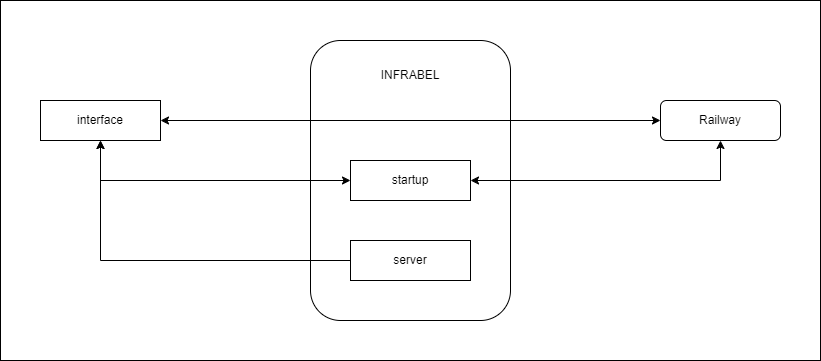
\includegraphics[scale=.5]{Afhankelijkheidsdiagrammen/infrabel.png}
\end{center}

\subsection{interface.rkt} % ++++++++++++++++++++++++++++++++++++++++++++++++++++++++++++++++++++++
De \texttt{Infrabel} klasse is het startpunt van de module en tevens ook de interface naar andere modules toe. Deze interface wordt opgeroepen vanuit een afzonderlijke file \texttt{INFRABEL.rkt}, deze voor de eindgebruiker gemakkelijk terug te vinden is.
\begin{table}[H]
	\begin{center}
		{\rowcolors{2}{gray!50!white!50}{white!100}
		\begin{tabular}{|l l l|}
			\hline
			\textbf{Naam} & \textbf{Signatuur} & \textbf{Uitleg}\\
			\hline
			\texttt{make-object} & (\empty \naar \textit{Infrabel}) & Constructor\\
			\hline
			\texttt{get-x} & (\textit{symbol} \naar \empty) & Placeholder voor getters voor uitwisseling van informatie\\
			\texttt{set-x!} & (\empty \naar \textit{symbol}) & Placeholder voor setters voor updaten van informatie\\
			\hline
		\end{tabular}}
		\caption{Operaties van de Infrabel/Main klasse}
	\end{center}
\end{table}

\subsubsection{startup.rkt} % ---------------------------------------------------------------------
De \texttt{Startup} klasse is de grafische representatie van het opstart menu, waar onder andere de configuratie voor de TCP verbinding zal kunnen gebeuren.
\begin{table}[H]
	\begin{center}
		{\rowcolors{2}{gray!50!white!50}{white!100}
		\begin{tabular}{|l l l|}
			\hline
			\textbf{Naam} & \textbf{Signatuur} & \textbf{Uitleg}\\
			\hline
			\texttt{make-object} & (\empty \naar \textit{Startup}) & Constructor\\
			\hline
		\end{tabular}}
		\caption{Operaties van de Infrabel/GUI/Startup klasse}
	\end{center}
\end{table}

\begin{comment}

\subsection{Logic} % ++++++++++++++++++++++++++++++++++++++++++++++++++++++++++++++++++++++++++++++

\subsubsection{App} % -----------------------------------------------------------------------------
De \texttt{App} klasse is verantwoordelijk voor de interne logica van de Infrabel module. Het besteet verschillende taken uit aan de klasses waarop deze steunt.
\begin{table}[H]
	\begin{center}
		{\rowcolors{2}{gray!50!white!50}{white!100}
		\begin{tabular}{|l l l|}
			\hline
			\textbf{Naam} & \textbf{Signatuur} & \textbf{Uitleg}\\
			\hline
			\texttt{make-object} & (\empty \naar \textit{App}) & Constructor\\
			\hline
			\texttt{get-x} & (\textit{symbol} \naar \empty) & Placeholder voor getters voor uitwisseling van informatie\\
			\texttt{set-x!} & (\empty \naar \textit{symbol}) & Placeholder voor setters voor updaten van informatie\\
			\hline
		\end{tabular}}
		\caption{Operaties van de Provider/Logic/App klasse}
	\end{center}
\end{table}

\end{comment}

\begin{comment}

\subsubsection{TCP} % -----------------------------------------------------------------------------
De \texttt{TCP} klasse is verantwoordelijk voor de communicatie met de Provider module.
\begin{table}[H]
	\begin{center}
		{\rowcolors{2}{gray!50!white!50}{white!100}
		\begin{tabular}{|l l l|}
			\hline
			\textbf{Naam} & \textbf{Signatuur} & \textbf{Uitleg}\\
			\hline
			\texttt{make-object} & (\empty \naar \textit{TCP}) & Constructor\\
			\hline
			\texttt{send-message} & (\textit{string} \naar \empty) & Verstuur een bericht naar de Provider module\\
			\hline
		\end{tabular}}
		\caption{Operaties van de Provider/Logic/TCP klasse}
	\end{center}
\end{table}

\end{comment}

\begin{comment}

\subsubsection{Collision-detector} % --------------------------------------------------------------
De \texttt{Collision-detector} klasse is verantwoordelijk voor het voorkomen van botsingen.
\begin{table}[H]
	\begin{center}
		{\rowcolors{2}{gray!50!white!50}{white!100}
		\begin{tabular}{|l l l|}
			\hline
			\textbf{Naam} & \textbf{Signatuur} & \textbf{Uitleg}\\
			\hline
			\texttt{make-object} & (\empty \naar \textit{Collision-detector}) & Constructor\\
			\hline
			\texttt{calculate-collision?} & (\textit{symbol} \textit{symbol} \naar \textit{boolen}) & Returnt mogelijke botsingen\\
			\hline
		\end{tabular}}
		\caption{Operaties van de Provider/Logic/Collision-detector klasse}
	\end{center}
\end{table}

\end{comment}

\begin{comment}

\subsubsection{Signalisator} % --------------------------------------------------------------------
De \texttt{Signalisator} klasse is verantwoordelijk dat alle signalisatie rondom de spoorweg correct is.
\begin{table}[H]
	\begin{center}
		{\rowcolors{2}{gray!50!white!50}{white!100}
		\begin{tabular}{|l l l|}
			\hline
			\textbf{Naam} & \textbf{Signatuur} & \textbf{Uitleg}\\
			\hline
			\texttt{make-object} & (\empty \naar \textit{Signalisator}) & Constructor\\
			\hline
			\texttt{update!} & (\textit{string} \naar \empty) & Update klasse met huidige staat spoorweg\\
			\hline
		\end{tabular}}
		\caption{Operaties van de Provider/Logic/Signalisator klasse}
	\end{center}
\end{table}

\end{comment}

\begin{comment}

\subsubsection{Concurrency} % ---------------------------------------------------------------------
De \texttt{Concurrency} klasse is verantwoordelijk voor het opstaan en inladen van de software.
\begin{table}[H]
	\begin{center}
		{\rowcolors{2}{gray!50!white!50}{white!100}
		\begin{tabular}{|l l l|}
			\hline
			\textbf{Naam} & \textbf{Signatuur} & \textbf{Uitleg}\\
			\hline
			\texttt{make-object} & (\empty \naar \textit{Concurrency}) & Constructor\\
			\hline
			\texttt{save} & (\textit{string} \naar \empty) & Slaat huidige staat van de software op.\\
			\texttt{load!} & (\textit{string} \naar \empty) & Laadt de staat van de software in van een bestand.\\
			\hline
		\end{tabular}}
		\caption{Operaties van de Provider/Logic/Concurrency klasse}
	\end{center}
\end{table}

\end{comment}

% =================================================================================================
\newpage
\section{Provider} % ==============================================================================
De Provider-module is een abstractie van de software die gebruikt kan worden door clienten (bijvoorbeeld NMBS). Deze module is verantwoordelijk voor het beheren van routes op het treinnetwerk, moet ervoor zorgen dat klanten correcte timetables hebben en het moet mogelijk zijn om na een crash de huidige staat van de fysieke spoorweg terug te krijgen.\\\\

\noindent \textbf{*** De provider module is nog niet ge\"implementeerd ***}\\

% =================================================================================================
\subsection{afhankelijkheidsdiagram} % ============================================================
\begin{center}
	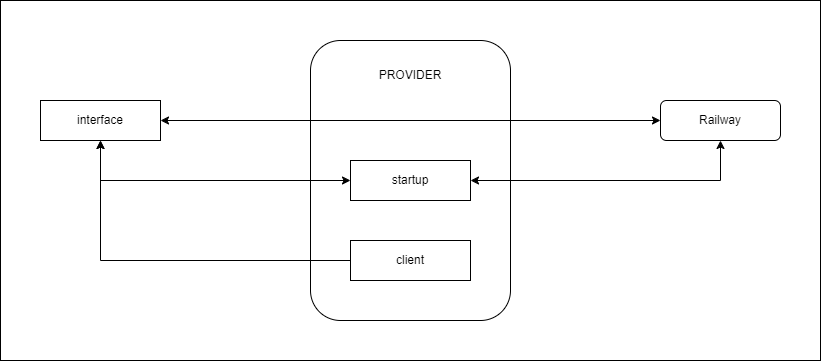
\includegraphics[scale=.5]{Afhankelijkheidsdiagrammen/provider.png}
\end{center}

\subsection{Main} % +++++++++++++++++++++++++++++++++++++++++++++++++++++++++++++++++++++++++++++++
De \texttt{Main} klasse is het startpunt van de module en tevens ook de interface naar andere modules toe. De module bestaat uit twee onafhankelijke delen, een Grafische User Interface (GUI) en de interne logica (Logic), waar de main-klasse de interface speelt tussen de twee.
\begin{table}[H]
	\begin{center}
		{\rowcolors{2}{gray!50!white!50}{white!100}
			\begin{tabular}{|l l l|}
				\hline
				\textbf{Naam} & \textbf{Signatuur} & \textbf{Uitleg}\\
				\hline
				\texttt{make-object} & (\empty \naar \textit{Provider}) & Constructor\\
				\hline
				\texttt{get-x} & (\textit{symbol} \naar \empty) & Placeholder voor getters voor uitwisseling van informatie\\
				\texttt{set-x!} & (\empty \naar \textit{symbol}) & Placeholder voor setters voor updaten van informatie\\
				\hline
		\end{tabular}}
		\caption{Operaties van de Provider/Main klasse}
	\end{center}
\end{table}

\subsubsection{Startup} % -------------------------------------------------------------------------
De \texttt{Startup} klasse is de grafische representatie van het opstart menu, waar onder andere de configuratie voor de TCP verbinding zal kunnen gebeuren.
\begin{table}[H]
	\begin{center}
		{\rowcolors{2}{gray!50!white!50}{white!100}
			\begin{tabular}{|l l l|}
				\hline
				\textbf{Naam} & \textbf{Signatuur} & \textbf{Uitleg}\\
				\hline
				\texttt{make-object} & (\empty \naar \textit{Startup}) & Constructor\\
				\hline
		\end{tabular}}
		\caption{Operaties van de Provider/GUI/Startup klasse}
	\end{center}
\end{table}

\begin{comment}

\subsubsection{Command\&Control} % ----------------------------------------------------------------
De \texttt{Command\&Control} klasse is de grafische user interface deze module, de gebruikers van de Provider zullen hier de volledige applicatie meer kunnen besturen.
\begin{table}[H]
	\begin{center}
		{\rowcolors{2}{gray!50!white!50}{white!100}
			\begin{tabular}{|l l l|}
				\hline
				\textbf{Naam} & \textbf{Signatuur} & \textbf{Uitleg}\\
				\hline
				\texttt{make-object} & (\empty \naar \textit{C\&C}) & Constructor\\\hline
				\texttt{update!} & (\empty \naar \empty) & Update de GUI naar de nieuwe staat van het systeem\\
				\hline
		\end{tabular}}
		\caption{Operaties van de Provider/GUI/Command\&Control klasse}
	\end{center}
\end{table}

\end{comment}

\begin{comment}

\subsubsection{TCP} % -----------------------------------------------------------------------------
De \texttt{TCP} klasse is verantwoordelijk voor de communicatie met de Infrabel module.
\begin{table}[H]
	\begin{center}
		{\rowcolors{2}{gray!50!white!50}{white!100}
			\begin{tabular}{|l l l|}
				\hline
				\textbf{Naam} & \textbf{Signatuur} & \textbf{Uitleg}\\
				\hline
				\texttt{make-object} & (\empty \naar \textit{TCP}) & Constructor\\
				\hline
				\texttt{send-message} & (\textit{string} \naar \empty) & Verstuur een bericht naar de Infrabel module\\
				\hline
		\end{tabular}}
		\caption{Operaties van de Provider/Logic/TCP klasse}
	\end{center}
\end{table}

\end{comment}

\begin{comment}

\subsubsection{Route-calculator} % ----------------------------------------------------------------
De \texttt{Route-calculator} klasse is verantwoordelijk voor het berekenen van de korste route tussen twee segmenten.
\begin{table}[H]
	\begin{center}
		{\rowcolors{2}{gray!50!white!50}{white!100}
			\begin{tabular}{|l l l|}
				\hline
				\textbf{Naam} & \textbf{Signatuur} & \textbf{Uitleg}\\
				\hline
				\texttt{make-object} & (\empty \naar \textit{Route-calculator}) & Constructor\\
				\hline
				\texttt{calculate-shortest-between} & (\textit{symbol} \textit{symbol} \naar \textit{pair}) & Berekent kortste route\\
				\hline
		\end{tabular}}
		\caption{Operaties van de Provider/Logic/Route-calculator klasse}
	\end{center}
\end{table}

\end{comment}

\begin{comment}

\subsubsection{Concurrency} % ---------------------------------------------------------------------
De \texttt{Concurrency} klasse is verantwoordelijk voor het opstaan en inladen van de software.
\begin{table}[H]
	\begin{center}
		{\rowcolors{2}{gray!50!white!50}{white!100}
			\begin{tabular}{|l l l|}
				\hline
				\textbf{Naam} & \textbf{Signatuur} & \textbf{Uitleg}\\
				\hline
				\texttt{make-object} & (\empty \naar \textit{Concurrency}) & Constructor\\
				\hline
				\texttt{save} & (\textit{string} \naar \empty) & Slaat huidige staat van de software op.\\
				\texttt{load!} & (\textit{string} \naar \empty) & Laadt de staat van de software in van een bestand.\\
				\hline
		\end{tabular}}
		\caption{Operaties van de Provider/Logic/Concurrency klasse}
	\end{center}
\end{table}

\end{comment}

\begin{comment}

\subsubsection{Timetables} % ----------------------------------------------------------------------
De \texttt{Timetables} klasse is verantwoordelijk voor het genereren van tijdstabellen.
\begin{table}[H]
	\begin{center}
		{\rowcolors{2}{gray!50!white!50}{white!100}
			\begin{tabular}{|l l l|}
				\hline
				\textbf{Naam} & \textbf{Signatuur} & \textbf{Uitleg}\\
				\hline
				\texttt{make-object} & (\empty \naar \textit{Timetables}) & Constructor\\
				\hline
				\texttt{generate-timetable} & (\textit{symbol} \naar \textit{pair}) & Genereert timetables voor trein\\
				\hline
		\end{tabular}}
		\caption{Operaties van de Provider/Logic/Timetables klasse}
	\end{center}
\end{table}

\end{comment}

% =================================================================================================
\label{lastpage}
\end{document}